\chapter{Locomotion with a Passive Mechanical Device}
\section{Motivation}

The bicycle was voted as the best invention since the 19th century \cite{BBC2005} because it is an inexpensive, fast, healthy and environmentally friendly mode of transportation. However, riding a bicycle is nontrivial due to its inherently unstable dynamics: The bike will fall without forward momentum and the appropriate human control. Getting onto the bike, balancing, steering and riding on bumpy roads all impose different challenges to the rider. As one important child development milestone, learning to ride a bicycle often requires weeks of practice. We are interested to find whether it is possible to use a computer to mirror this learning process. In addition to the basic maneuvers, the most skillful riders can jump over obstacles, lift one wheel and balance on the other, and perform a large variety of risky but spectacular bicycle stunts. Performing stunts requires fast reaction, precise control, years of experience and most importantly, courage, which challenges most people. Can we design an algorithm that allows computers to automatically learn these challenging but visually exciting bicycle stunts?

Designing an algorithm to learn to ride a bicycle presents unique challenges. Riding a bicycle involves complex interactions between a human rider and a bicycle. While the rider can actively control each joint, the bicycle is a passive system that can only be controlled by the human rider. To control a single degree of freedom (DOF) of a bicycle, coordinated motions of multiple DOFs of the rider are required. Moreover, the main difficulty in locomotion is to control an under-actuated system by exploiting external contact forces. Manipulating contact forces on a bicycle is indirect. All of the rider's control forces need to first go through the bicycle dynamics to affect the ground reaction forces and vice versa. This extra layer of bicycle dynamics between the human control and the contact forces adds another layer of complexity to the locomotion control. Balance on a bicycle is challenging and it is different from balance when standing or walking. While a human can stand stably due to the large contact area of the feet, a static bicycle cannot stay upright due to its narrow tires. Humans can balance during walking by planning and changing their foot placement. In contrast, the bike rider cannot abruptly change the contact position, which can only be changed gradually through steering. The limited range of human motion on a bicycle makes balance even harder. When the character's hands are constrained to hold the handlebar and their feet are on the pedals, the character loses much of the freedom to move various body parts. He or she cannot employ ankle or hip postural strategies or wave their arms to effectively regulate the linear and the angular momenta.

Balance during bicycle stunts is far more challenging than normal riding. As a stunt example that illustrates the balance issues we plan to tackle, consider a bicycle endo (bottom-left image of Figure~\ref{fig:teaser3}), in which the rider lifts the rear wheel of the bicycle and keeps balance on the front wheel. In this pose, the rider encounters both the longitudinal and lateral instabilities. The small contact region of one wheel and the lifted center of mass (COM) due to the forward leaning configuration exacerbate the balance problem. Furthermore, the off-the-ground driving wheel makes any balance strategies that involve acceleration impossible. The unstable configurations and the restricted actions significantly increase the difficulty of balance during a stunt.

This paper describes a complete system for controlling a human character that is riding a bicycle in a physically simulated environment. The system consists of two main components: simulating the motion and optimizing the control policy. We simulate the bicycle and the rider as an articulated rigid body system, which is augmented with specialized constraints for bicycle dynamics. The second component provides an automatic way to learn control policies for a wide range of bicycle maneuvers. In contrast to many optimal control algorithms that leverage the dynamics equations to compute the control signals, we made a deliberate choice not to exploit the dynamics equations in our design of the control algorithm. We believe that learning to ride a bicycle involves little reasoning about physics for most people. A four-year-old can ride a bicycle without understanding any physical equations. Physiological studies show that learning to ride a bicycle is a typical example of implicit motor learning \cite{Chambaron2009}, in which procedural memory guides our performance without the need for conscious attention. Procedural memory is formed and consolidated through repetitive practice and continuous evolution of neural processes. Inspired by the human learning process, we formulate a partially observable Markov decision process (POMDP) and use policy search to learn a direct mapping from perception to reaction (procedural memory).

Both prior knowledge of bicycle stunts and an effective searching algorithm are essential to the success of policy search. After studying a variety of stunts, we classify them into two types. We apply feed-forward controllers for the \emph{momentum-driven} motions and feedback controllers for the \emph{balance-driven} ones. We study videos of stunt experts to understand their reactions under different situations and used this information to design the \emph{states} and the \emph{actions} of our controllers. We employ a neural network evolution method to simultaneously optimize both the parametrization and the parameters of the feedback controllers. The way we incorporate the prior knowledge into our system and the effective evolutionary method are both essential to the success of policy search.

We evaluate our system by demonstrating a human character riding different types of bicycles and performing a wide variety of stunts (Figure \ref{fig:teaser3}). We also evaluate the importance of optimizing the parametrization of a policy. We share our experiences with different reinforcement learning algorithms that we have tried throughout this research project.

\section{Related Work}
Prior research that inspired our work include techniques from character locomotion control, the study of bicycle dynamics, and algorithms in reinforcement learning. We will review the work in each of these sub-areas in turn.

\paragraph{Character locomotion control.} Controlling character locomotion in a physically simulated environment has been extensively studied in both computer animation and robotics. Researchers have investigated different forms of locomotion, including walking \cite{Yin:2007,Wang:2012}, running \cite{Hodgins:1995:AHA,Kwon:2010}, flying \cite{Wu:2003} and swimming \cite{Grzeszczuk:1995,Tan:2011}. One central problem of locomotion is balance, which can be controlled by exerting virtual forces \cite{Pratt2001,Coros2010}, applying linear feedback \cite{Laszlo:1996,Yin:2007,daSilva:2008,Coros2010}, using nonlinear control policies \cite{Muico:2009}, planning the contact forces \cite{Muico:2009,Tan:2012}, employing reduced models \cite{Tsai:2010,Kwon:2010,mordatch2010,Coros2010,Ye:2010} and training in stochastic environments \cite{Wang:2010}. Among many different techniques, Covariance Matrix Adaptation Evolution Strategy (CMA-ES) \cite{Hansen:2009} is one of the most frequently applied optimization methods for locomotion control. We use CMA to optimize the control policies for momentum-driven bicycle maneuvers.

Compared to walking and running, fewer studies focus on locomotion that involves a character that is controlling another device with complex dynamics. Van de Panne and Lee \cite{vandepanne:2003} built a 2D ski simulator and that relies on user inputs to control the character. This work was later extended to 3D by Zhao and Van de Panne \cite{Zhao:2005}. Planar motions, including pumping a swing, riding a seesaw and even pedaling a unicycle, were studied \cite{Hodgins:1992}. Hodgins et al. \cite{Hodgins:1995:AHA} demonstrated that normal cycling activities, including balance and steering, can be achieved using simple proportional-derivative (PD) controllers for the handlebar angle. These linear feedback controllers are sufficient for normal cycling, but they cannot generate the bicycle stunts demonstrated in this paper.

Our system resembles stimulus-response control proposed in several early papers. Van de Panne and Fiume \cite{vandePanne:1993} optimized a neural network to control planar creatures.
Banked Stimulus Response and genetic algorithms were explored to animate a variety of behaviors for both 2D \cite{Ngo:1993} and 3D characters \cite{Auslander:1995}. Sims \cite{Sims:1994} used genetic programming to evolve locomotion for virtual creatures with different morphologies. Contrary to the general belief that the stimulus-response framework does not scale well to high-dimensional models and complex motions \cite{Geijtenbeek2012a}, we demonstrate that this framework can indeed be used to control a human character performing intricate motions.

\paragraph{Bicycle dynamics.} Early studies of bicycle dynamics date back to more than a century ago. As described in Meijaard et al. \cite{Meijaard2007}, Whipple \cite{Whipple1899} and Carvallo \cite{Carvallo1900} independently derived the first governing equations of bicycle dynamics. These equations were revised to account for the drag forces \cite{Collins1963}, tire slip \cite{Singh1964} and the presence of a rider \cite{van1975method}. Rankine \cite{Rankine1870} discussed the balance strategy of ``steering towards the direction of falling'', which forms the foundation of many studies on bicycle balance control, including ours. Despite this long history of research and the seemingly simple mechanics of bicycles, some physical phenomena exhibited by the bicycle movement still remain mysterious. One example is the self-stable characteristic of bicycles: A moving bicycle within a narrow range of forward speed can automatically correct its falling motion without any human intervention. In addition to the early belief that this phenomenon was attributed to gyroscopic effects of the rotating wheels \cite{Klein1910} or the \emph{trail}\footnote{The trail is the distance between the front wheel ground contact point and the steering axis.} \cite{Jones1970}, Kooijman et al. \cite{Kooijman2011} showed that the mass distribution over the whole bicycle also contributes to the self-stability. Even though the dynamic equations provide us with some intuition, we do not use this information directly in our algorithm because this is tailored specifically to normal riding situations where both tires touch the ground. This will be a major restriction in bicycle stunts.

\paragraph{Reinforcement learning.} The bicycle control problem can be formulated and solved as a reinforcement learning problem. Value iteration is a widely-used reinforcement learning algorithm in computer graphics. Researchers have successfully applied (fitted) value iteration to generalize motion capture data \cite{Treuille:2007:NCA,Levine:2012:CCC}, to carry out locomotion tasks \cite{Coros:2009:RTC}, and to manipulate objects with hands \cite{Multifinger2013}. Applying value iteration to continuous state and action spaces is nontrivial because discretizing the space does not scale well to high dimensions \cite{Sutton:1998:IRL} and using function approximation often converges to a poor local minimum or might not converge at all \cite{Thrun93issuesin,Boyan95generalizationin}. Policy search \cite{Ng:2000:PPS} is another reinforcement learning algorithm, which directly searches for a mapping between the state space and the action space. Many studies on locomotion control \cite{Yin08,Wang:2009,Coros:2011,Tan:2011,Wang:2012,Geijtenbeek:2013} performed policy search on parameterized controllers.

The bicycle control problem has been investigated in the reinforcement learning literature. Randl$\o$v and Alstr$\o$m \cite{RandlovAlstrom:1998} used SARSA($\lambda$), a model free reinforcement learning algorithm, to learn to balance a bicycle and ride to a goal. This algorithm requires a large number of simulation trials and the converged result is still not ideal. Ng and Jordan \cite{Ng:2000:PPS} applied policy search to the same bicycle learning problem. They parameterized the policy with neural networks and used the policy gradient to find the optimal network weights. The resulting controller significantly outperformed the results in the previous study. Our method is inspired by the policy search algorithm. However, to adopt this algorithm to learn more challenging tasks, we need to overcome two difficulties: First, we do not have reliable policy gradient information because of the frequent contact events. Second, we do not know a good policy parametrization, which is difficult to design manually by trial and error for each bicycle stunt. We use NEAT \cite{Stanley:2002:ENN} which was first introduced to graphics by Allen and Faloutsos \cite{Allen2009}, to address both difficulties. NEAT was first introduced to graphics by Allen and Faloutsos \cite{Allen2009}. They used it to evolve locomotion controllers but were not able to achieve stable and sustained walking. We show in this paper that With appropriate choices of the states and actions, combining policy search with NEAT can successfully learn the most demanding balance tasks on a bicycle. Please read Section ~\ref{sec:improvement} for more details about NEAT.

\section{Overview}
\begin{figure}[!t]
  \centering
  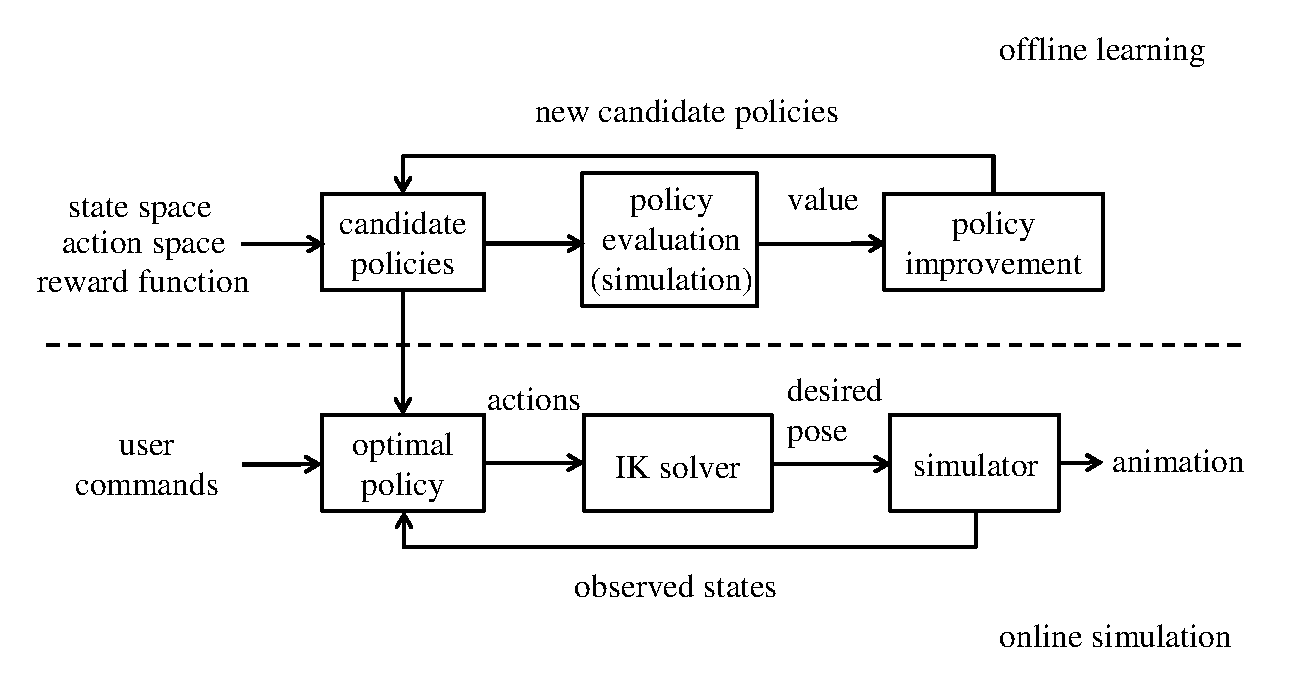
\includegraphics[width=3.4in]{figures/overview}
  \caption{Overview of our algorithm.}
  \vspace{-0.1in}
  \label{fig:overview}
\end{figure}

We have designed a system that allows a virtual human character to learn to ride a bicycle and perform a wide variety of stunts. The goal of our system is to learn a control policy that initiates a particular action at any state. Given the state space, the action space and the reward function for each bicycle task, the offline learning subsystem starts with an initial set of candidate policies, iteratively evaluates (using simulation) and evolves them (using CMA or NEAT) until the optimal policy is found. This optimal policy allows the user to interact with the bicycle simulation in real time by giving commands such as steering to the left. The online simulation subsystem first extracts the observable states, such as the tilt angle, the falling speed, and the actual and the user-specified handlebar angle. It then queries the policy to determine appropriate actions, such as turning the handlebar at a certain speed to fulfill the user's command while still maintain the balance of the bicycle. Executing actions, such as turning the handlebar, requires a coordinated full-body motion of the rider. An Inverse Kinematics (IK) solver maps the compact set of actions to the rider's full-body pose. The simulator tracks this desired pose and at the same time simulates the dynamics of both the human rider and the bicycle. Figure \ref{fig:overview} illustrates the main components of our system.

\section{Bicycle and Rider Simulation}
Our simulator is based on Open Dynamic Engine (ODE) \cite{ode:2008},
but we augmented it with additional constraints to simulate both the
bicycle and the human rider. We treat the bicycle and the rider as a
system of articulated rigid bodies. Since the dynamics is represented
in the maximal coordinates, each rigid body has six DOFs and its
dynamic equation is
\begin{equation}
\left[\begin{array}{cc}
\vc{M} & \vc{0} \\
\vc{0} & \vc{I}
\end{array}\right]
\left[\begin{array}{c}
\dot{\vc{v}} \\
\dot{\vc{\omega}}
\end{array}\right]=
\left[\begin{array}{c}
m\vc{g} \\
-\dot{\vc{I}}\vc{\omega}
\end{array}\right]
+\vc{J}^T
\left[\begin{array}{c}
\vc{f}\\
\vc{\tau}
\end{array}\right]
\label{eq:dynamics}
\end{equation}
where $\vc{M}$ is the mass matrix, $\vc{I}$ is the inertia tensor, $\vc{v}$ and $\vc{\omega}$ are the linear and angular velocities, $\vc{f}$ and $\vc{\tau}$ are the constraint forces and torques, which come from the bicycle chains, the joints, the actuators and the contacts. $\vc{J}^T$ is the transposed Jacobian matrix that maps the constraint forces and torques to the body.

Chains transfer power from the pedals to the rear wheel on a bicycle. We use a linear equality constraint to realize the effect of a bicycle chain.
\begin{equation}
\vc{n}^T(\alpha\vc{\omega}_A-\vc{\omega}_B)=0
\label{eq:chainConstraint}
\end{equation}
where bodies $A$ and $B$ are the pedals and the rear wheel. $\vc{n}$ is the common direction of their rotational axes and $\alpha$ represents the gear ratio, which is the ratio between the number of teeth on the chain-ring and the number on the rear sprocket. Note that Equation~(\ref{eq:chainConstraint}) models a fixed-gear bicycle. In some tasks, we disabled this constraint to mimic the effect of the free wheel, allowing the rider to glide without pedaling.

The other constraints are standard from the implementation of ODE. For completeness of presentation, we include a brief description of such constraints in the supplementary material. Note that we use the actuator constraints instead of the traditional PD servos to track a desired pose. We have found that using the actuator constraints enables us to simulate at large time steps (0.01s), which significantly speeds up the computation.

We made several simplifications in the simulation. We used ball joints to attach the rider's feet to the pedals. This treatment is similar to wearing toe clips in the real world. We also used ball joints to connect the rider's hands with the handlebar. For some tasks in which the rider is seated, we further constrained the relative position and orientation between the rider's pelvis and the bicycle seat.


\section{Learning to Ride a Bicycle}
\label{sec:control}

\subsection{Markov Decision Process}
We formulate the bicycle control problem as a POMDP. A Markov decision process (MDP) is a tuple $(S, A, R, D, P_{sas'}, \gamma)$, where $S$ is the \emph{state} space; $A$ is the \emph{action} space; $R$ is the \emph{reward function}; $D$ is the distribution of the initial state $s_0$; $P_{sas'}$ is the transition probability; and $\gamma \in [0, 1]$ is the discount factor. For example, in the bicycle balance task, we choose the state space $S$ to include the tilt angle of the bike, the tilting speed and the handlebar angle. We choose the action $A$ to be turning the handlebar at a certain speed. We choose the reward function $R$ at the state $s$ to be
\begin{equation}
\begin{array}{ll}
R(s) = & \left\{ \begin{array}{ll}
1 & \textrm{if the bicycle remains upright,}\\
0 & \textrm{otherwise.}
\end{array} \right. \\
\end{array}
\label{eq:balanceReward}
\end{equation}
The initial state $s_0$ is drawn from a random perturbation near the upright orientation of the bicycle. The state transition is calculated using simulation, and we do not discount the rewards ($\gamma = 1$).

A \emph{policy} is a mapping from states to actions: $\pi : S \mapsto A$. The \emph{return} of a policy is the accumulated rewards along the state trajectory starting at $s_0$ by following the policy $\pi$ for $N$ steps.
\begin{displaymath}
V^\pi(s_0)=\sum_{i=0}^N{R(s_i)}
\end{displaymath}
The \emph{value} of a policy is the expected return with respect to the random initial state $s_0$ drawn from D.
\begin{equation}
V(\pi)=E_{s_0\sim D}[V^\pi(s_0)]
\label{eq:policyValue}
\end{equation}
The optimal solution of an MDP is the policy that has the maximum value $\pi^*=\arg\max_\pi V(\pi)$. The optimal policy in the bicycle balance example decides how to turn the handlebar under different situations so that the bicycle can stay upright for the longest time.

Our MDP is partially observable because we choose to observe only a selected subset of all the simulation states. We have found that focusing on a small number of relevant states for each task results in a more efficient learning process. The actions are also selected based on our prior knowledge of the task. Table~\ref{table:states} and~\ref{table:actions} summarize all the states and actions used across our different examples. The 25 states in Table~\ref{table:states} may seem exhaustive, but we only use a subset of them (typically not more than eight states) for each task.

\begin{table}[!t]
\centering
\begin{tabular}{|l|l|}
\hline
state & description \\
\hline
$t$    & time (used in the feed-forward controllers)\\
$\theta$ & handlebar angle \\
$\alpha$    & roll angle of the bike (tilt left/right)   \\
$\dot{\alpha}$     & roll speed  \\
$\beta$     & pitch angle of the bike  \\
$\dot{\beta}$     & pitch speed  \\
$\gamma$     & yaw angle of the bike \\
$\dot{\gamma}$ & yaw speed \\
$v_r$ & rear wheel linear speed \\
$v_f$    & front wheel linear speed  \\
$h_r$     & rear tire height above the ground  \\
$h_f$     & front tire height above the ground  \\
$x$    & pelvis position along x-axis\\
$y$    & pelvis position along y-axis\\
$z$    & pelvis position along z-axis\\
$\phi$    & torso orientation in the Sagittal plane\\
$\psi$    & torso orientation in the Coronal plane\\
$\chi$   & torso orientation in the Transverse plane\\
$\dot{\phi}$    & torso angular speed in the Sagittal plane\\
$\dot{\psi}$    & torso angular speed in the Coronal plane \\
$\dot{\chi}$   & torso angular speed in the Transverse plane\\
$\Delta\theta $ & difference between actual and desired handlebar angle \\
$\Delta\beta$    & difference between actual and desired pitch angle\\
$\Delta v_r $ & difference between actual and desired rear wheel speed \\
$\Delta v_f $ & difference between actual and desired front wheel speed \\
\hline
 \end{tabular}
 \caption{States and their descriptions. The rider's pelvis position, torso orientation and angular velocity are calculated in the bicycle frame's coordinates.}
 \vspace{-0.1in}
 \label{table:states}
 \end{table}

\begin{table}[!t]
  \centering
\begin{tabular}{|l|l|}
\hline
action & description \\
\hline
$\dot{\theta}$ & steering\\
$\dot{v}_r $ & accelerating or braking\\
$\dot{v}_f $ & accelerating or braking on a front-wheel-driven bicycle\\
$\tau_f$    & front braking   \\
$\dot{x}$     & pelvis motion along x-axis\\
$\dot{y}$     & pelvis motion along y-axis\\
$\dot{z}$     & pelvis motion along z-axis\\
$\dot{\phi}$    & torso motion in the Sagittal plane\\
$\dot{\psi}$    & torso motion in the Coronal plane \\
$\dot{\chi}$   & torso motion in the Transverse plane\\
$\tilde{x}$     & desired pelvis position along x-axis\\
$\tilde{y}$     & desired pelvis position along y-axis\\
$\tilde{z}$     & desired pelvis position along z-axis\\
$\tilde{\phi}$    & desired torso orientation in the Sagittal plane\\
\hline
\end{tabular}
\caption{Actions and their descriptions. The rider's pelvis and torso movements are relative to the bicycle frame's coordinates.}
\vspace{-0.1in}
\label{table:actions}
\end{table}


\subsection{Policy Search}
We apply policy search to optimize the control policies. Unlike value iteration, policy search can be easily applied to MDPs in high dimension and with continuous state and action spaces. This algorithm searches for the optimal policy within a parameterized functional space $\pi^*\in\Pi$. During policy search, one or more random policies are generated as an initial guess. These candidates are evaluated and improved iteratively. Policy improvement can be guided using the policy gradient \cite{Ng:2000:PPS}, trajectory optimization \cite{Levine2013} or other optimization techniques \cite{Heidrich-Meisner:2008}. Policy search ends when the iteration converges or the maximum number of iterations is reached.

\begin{figure*}[!t]
\centering
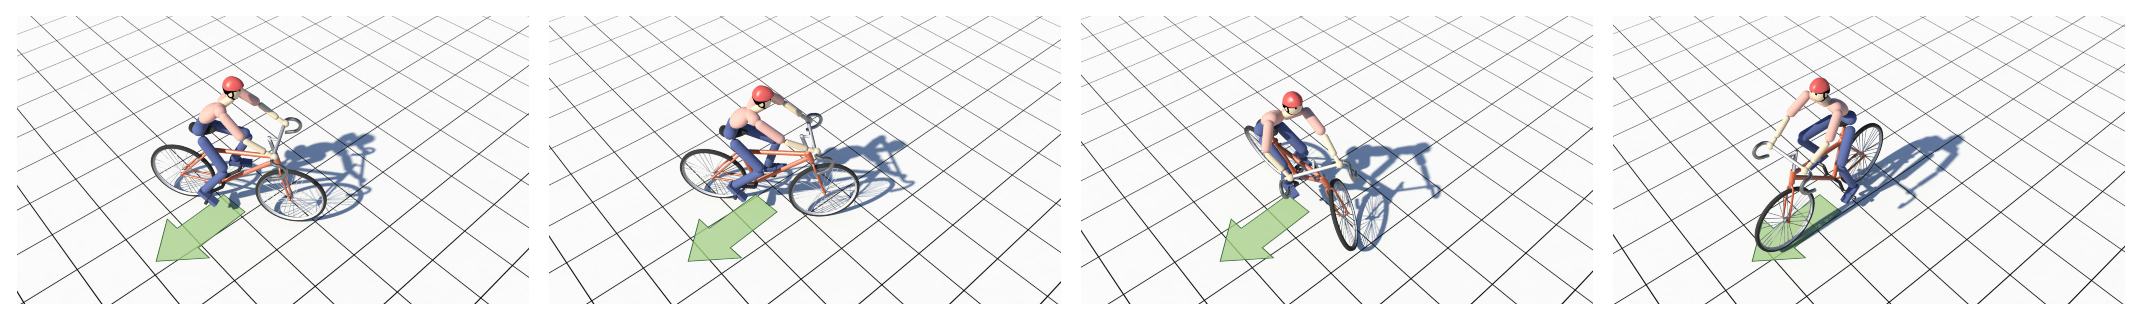
\includegraphics[width=\textwidth]{figures/maneuver}
\caption{A character steers the road bike towards the green arrow.}
\label{fig:balance}
\end{figure*}

\begin{figure*}[!t]
\centering
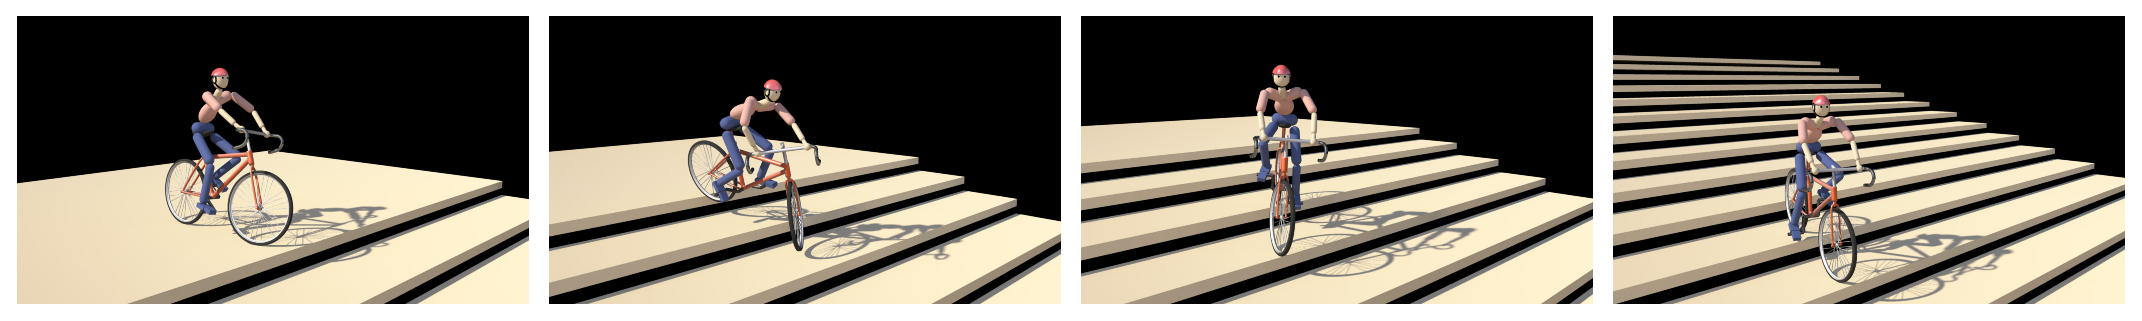
\includegraphics[width=\textwidth]{figures/staircase}
\caption{A character rides down a set of stairs without falling over.}
\vspace{-0.1in}
\label{fig:stair}
\end{figure*}

\subsubsection{Policy Parametrization}
\label{sec:parametrization}

\begin{figure}[!t]
  \centering
  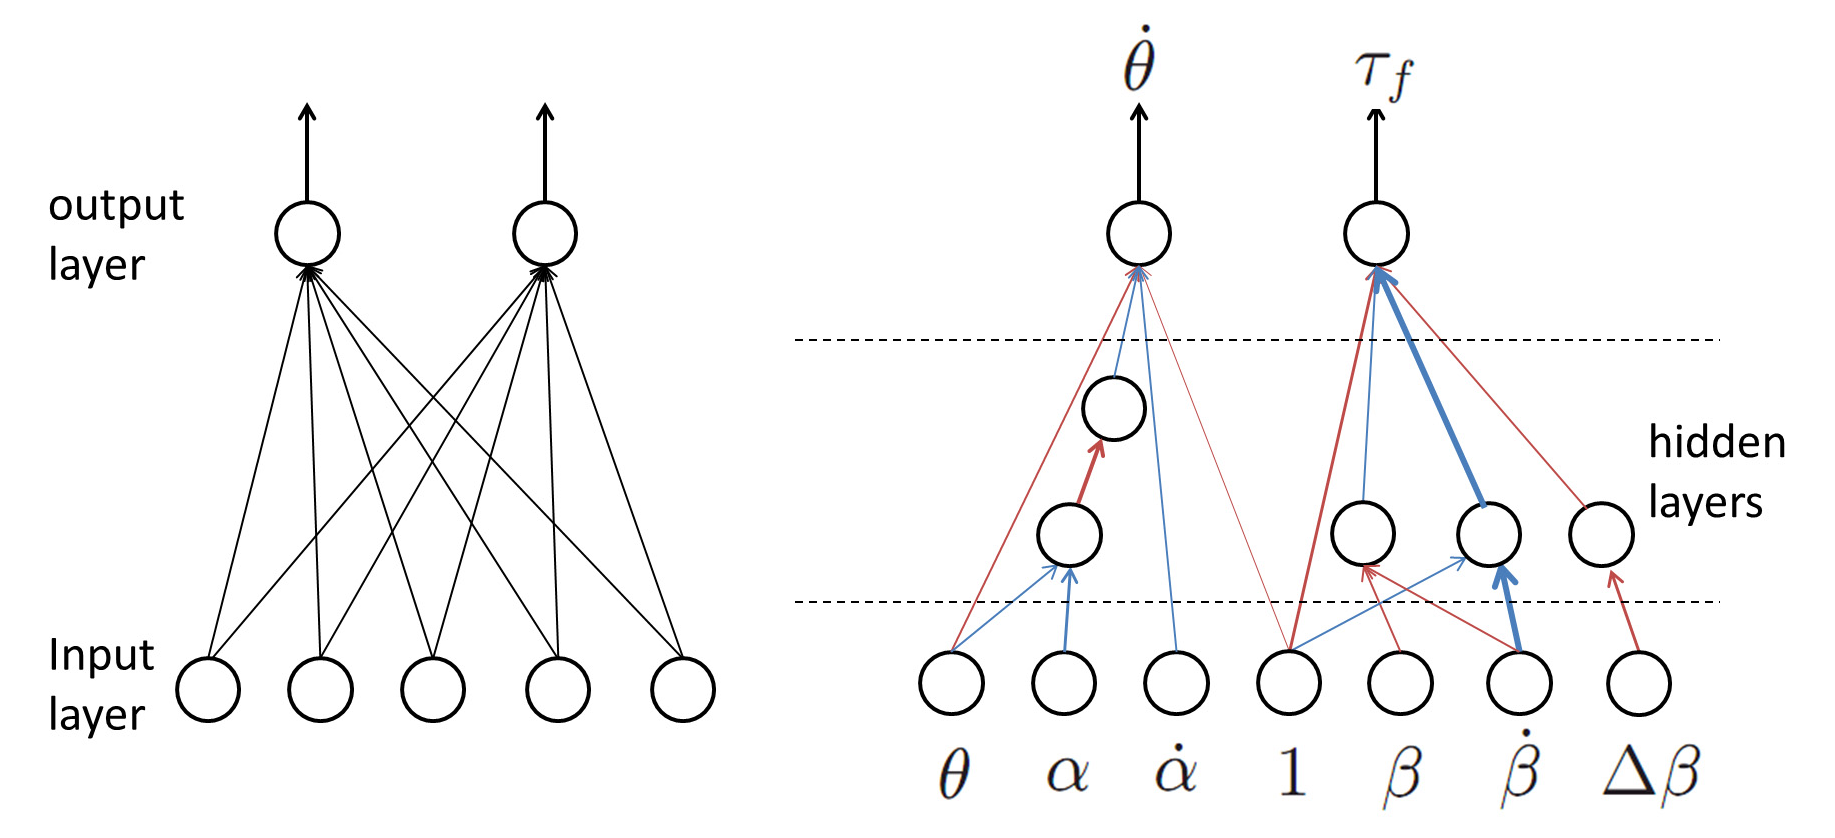
\includegraphics[width=3.4in]{figures/simpleNetwork}
  \caption{Left: A simple neural network with input and output layers that are directly connected. Right: A neural network learned using our algorithm for balancing on the front wheel. Blue arrows mean negative weights while red mean positive weights. The width of the arrows encodes the magnitude of the weights. }
  \vspace{-0.1in}
  \label{fig:simpleNetwork}
\end{figure}

We use two types of parametrizations for the bicycle control problem: splines for feed-forward control and neural networks for feedback control. We found that most of the stunts can be categorized into momentum-driven, balance-driven or a combination of the two. The momentum-driven stunts involve vigorous full body motions to manipulate the bicycle to a desired orientation. Coordinated full body motions with large magnitude are essential, but the short duration of this type of stunts makes balance easy to maintain. For this reason, we use feed-forward controllers and represent the action trajectories as cubic Hermite splines. Assuming that the number of control points is given, the parameters to optimize are the time and the value of the control points\footnote{We do not optimize the tangents at the control points and we set them to be zero.}.

Balance-driven stunts require that the rider carefully adjusts his or her COM and maintains a stunt pose for a longer period of time. Feedback balance control is vital to the duration of the performance, which determines the success or failure of the stunt. We use neural networks for their ability to approximate a wide range of functions. The inputs to a network are the observed states, and the outputs are the actions. Figure~\ref{fig:simpleNetwork} Left illustrates a simple neural network that directly connects the input and the output layers. The output of neuron $i$ is
\begin{displaymath}
v_i=\sigma(\sum_j w_{ij} v_j)
\end{displaymath}
where $w_{ij}$ is the connection weight between neuron $i$ and $j$, and $\sigma$ is the sigmoid function $\sigma(x) = 1/(1+e^{-x})$.

Parametrization determines the potential quality of the optimal policy. The network shown in Figure~\ref{fig:simpleNetwork} Left is too simple for representing a complex policy required by bicycle stunts. However, it is not clear how to manually design the network structure, given the control policies of unsuccessful stunts. For this reason, we use NEAT to search for both the structure of the neural network and its weights simultaneously, which finds far better policies than searching over a fixed network. Figure~\ref{fig:simpleNetwork} Right demonstrates the learned network for the balance task of a bicycle endo using NEAT. See Section~\ref{sec:improvement} for more details.

\subsubsection{Policy Evaluation}
To evaluate a policy, we formulate a reward function in the following form:
\begin{equation}
R(s)=R_t(s)+wR_r(s)
\end{equation}
where $R_t$ and $R_r$ are task-specific and regularization terms respectively. $w$ is the weight.

We use eq.(\ref{eq:balanceReward}) as the task-specific reward for balance-driven tasks. As the reward is accumulated over time, the return counts the number of frames that the bicycle stays upright. The task-specific reward varies for each momentum-driven stunt. For example, the reward for initiating an endo (lifting the rear wheel) is to maximize the negative pitch angle of the bike $R_t=-\beta$. We refer the readers to Section \ref{sec:results} and for more detailed descriptions of task-specific rewards.

Given the task-specific reward term alone, multiple optimal policies could exist. Taking the balance task as an example, a policy that rides in a straight line and another that oscillates in a sinusoidal path by periodically swinging the handlebar can both balance well and thus yield the same value. The regularization term is mainly used to eliminate this ambiguity. We use the regularization term $R_r=\frac{1}{|\theta|+\epsilon}$ to express our preference of riding straight. In our examples, all the regularizers are in the form of
\begin{displaymath}
R_r = \frac{1}{|X|+\epsilon}
\end{displaymath}
where $X$ can be substituted by $\alpha$ for the upright bicycle position, $\Delta \theta$ for the desired steering angle, $\Delta \beta$ for the desired pitch angle, $\Delta v$ for the desired speed, $(x, y, z)$ and $(\phi, \psi, \chi)$ for small changes of rider's pelvis position and torso orientation. A small number $\epsilon$ in the denominator is used to bound the reward.

We do not explicitly minimize the rider's effort in the reward function because it is difficult to balance the effort minimization objective and the task-specific objective for difficult stunt actions. However, we limit the maximum actuated joint torques of the rider in the simulation to ensure that the rider does not possess super-human strength.

We run multiple simulations with different initial configurations $s_0$, which are sampled from random perturbations of the default bicycle velocity and orientation, to evaluate the value of a policy. At each simulation step, our algorithm calculates the reward for the current state, and accumulates this until the bicycle falls or after 1000 time steps. The average return of all the simulations is the value of the policy.

\begin{figure*}[!t]
\centering
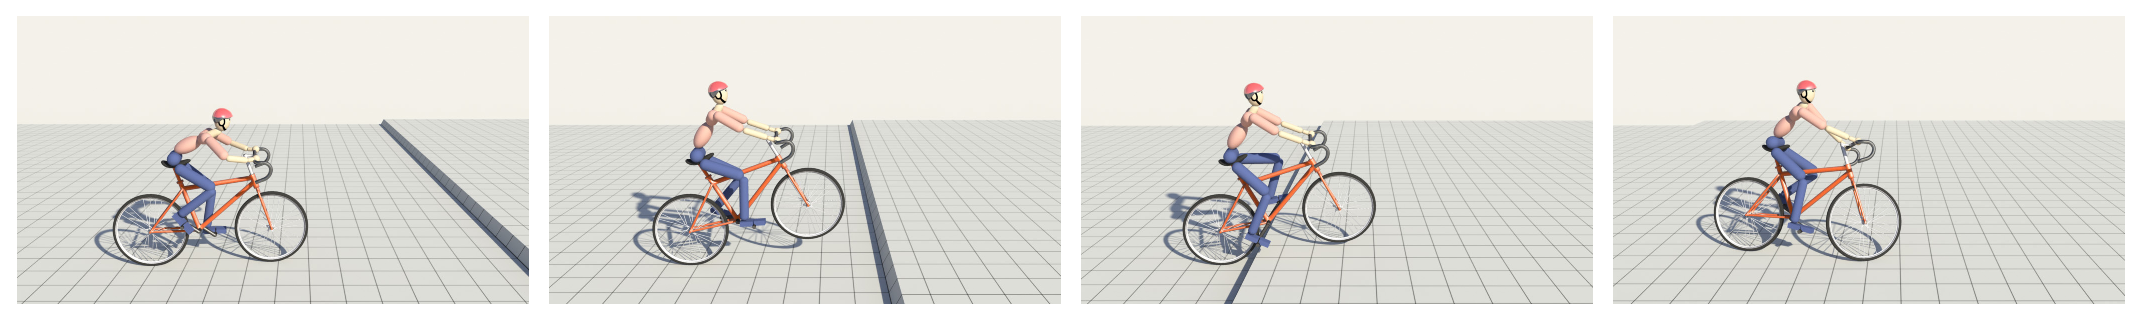
\includegraphics[width=\textwidth]{figures/Curb}
\caption{A character lifts the front wheel to ride over a curb.}
\label{fig:curb}
\end{figure*}

\begin{figure*}[!t]
\centering
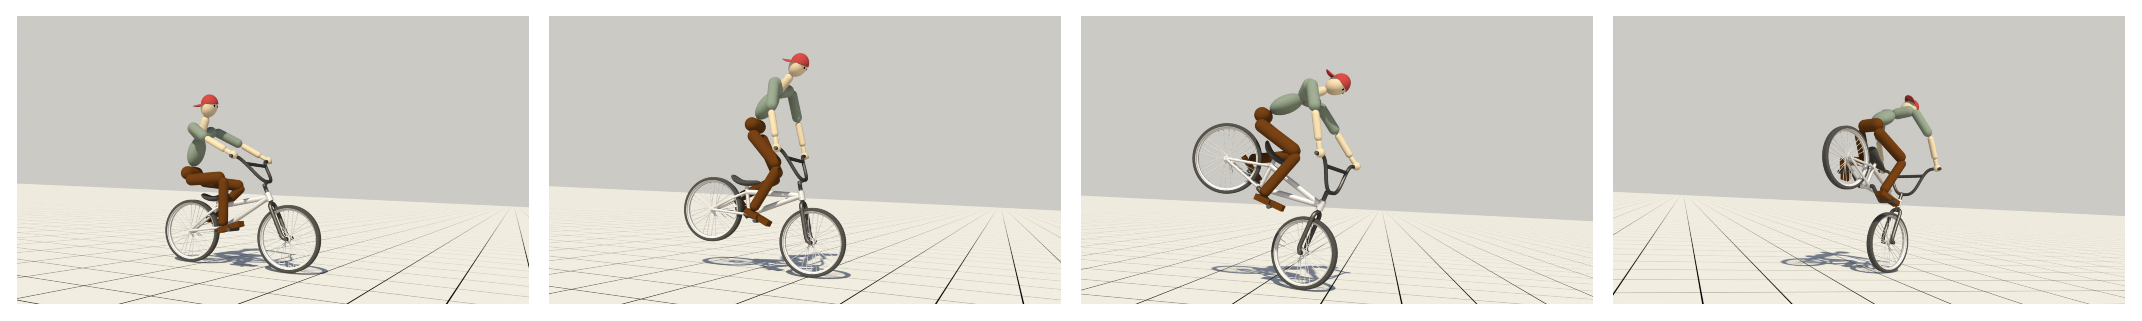
\includegraphics[width=\textwidth]{figures/endo}
\caption{A character performs an endo and balance on the front wheel.}
\vspace{-0.1in}
\label{fig:endo}
\end{figure*}

\subsubsection{Policy Improvement}
\label{sec:improvement}

Many policy improvement methods utilize the policy gradient \cite{Peters:2008} to perform iterative ascending operations. However, our simulation of bicycle stunts involves frequent discrete events such as establishing and breaking contact, which invalidates the gradient information. For this reason, we use sample-based stochastic optimization techniques. We apply CMA to search for the feed-forward controllers since the parametrization of splines is fixed. We use NEAT to search for feedback controllers, including the structure and the weights of the neural network. NEAT has many similarities to genetic algorithms, but it is tailored to the creation of neural networks. We will describe NEAT briefly below. For further details we refer readers to the original paper \cite{Stanley:2002:ENN}.

NEAT iteratively performs evaluation, selection, crossover and mutation. To maximize the value of a policy, NEAT starts with a simple network structure, in which the input and the output layers are directly connected. A population of such networks with random weights is drawn as an initial guess. These candidate policies are evaluated and the top 20\% are selected to survive. Pairs of randomly-selected surviving policies are crossed over to produce a new generation (more on this below). Mutations (with low probability) can perturb connection weights, add a neuron or add a connection. Note that the addition of a neuron or a connection complexifies the network structure and enriches the class of functions that it can represent.

Crossover is nontrivial in NEAT because the parent neural networks can have different topologies. To overcome this difficulty, the newly-added neuron or connection is assigned a unique innovation number, which tells the history of the mutation and how to match up neurons or connections between parents during crossover. The neurons or connections that share the same innovation number across parents are from the same ancestor, which will be inherited randomly by the child sample. The neurons or connections that have no counterparts in the other parent are from different mutations. They will be inherited from the parent with the higher value.

The evolution ends when the policy values do not increase over a certain number of iterations or the maximum number of iterations is reached.

\section{Results}
\label{sec:results}

\begin{figure*}[ht]
\centering
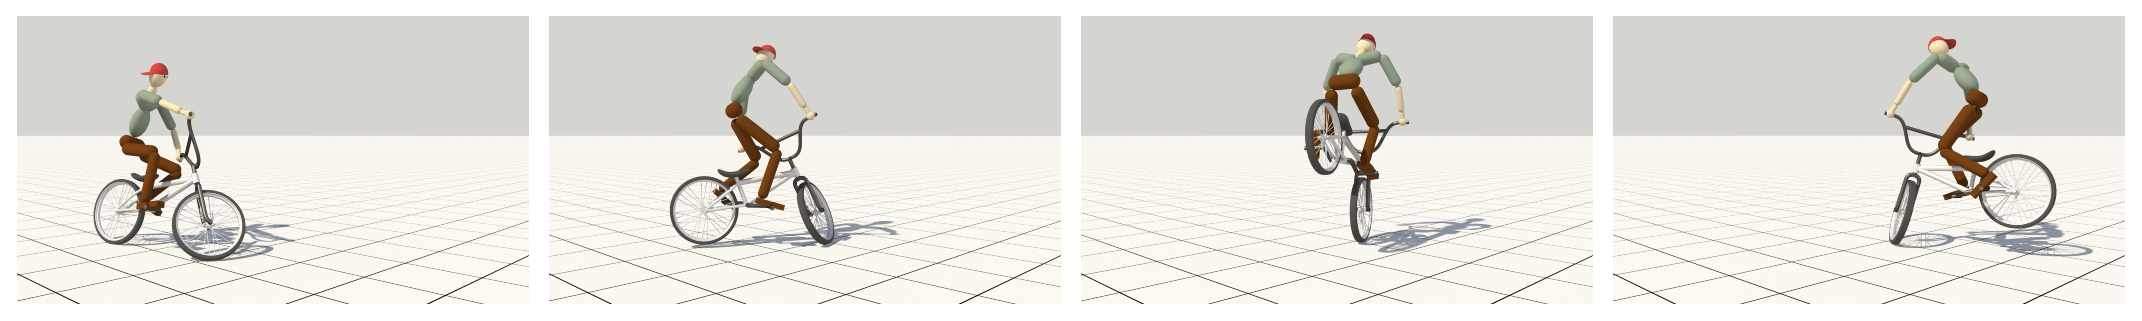
\includegraphics[width=\textwidth]{figures/frontWheelPivot}
\caption{A character completes a quick 180-degree turn by pivoting the bicycle on the front wheel.}
\label{fig:pivot}
\end{figure*}


\begin{figure*}[ht]
\centering
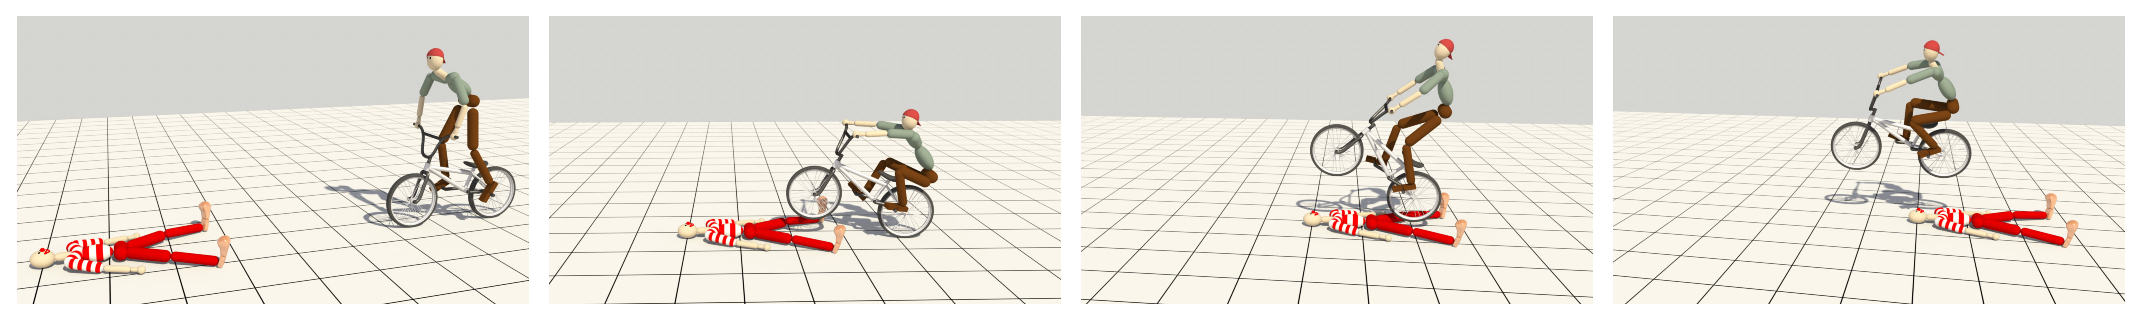
\includegraphics[width=\textwidth]{figures/bunnyHop}
\caption{A character performs the American bunny hop over a clown lying on the ground.}
\vspace{-0.1in}
\label{fig:bunnyhop}
\end{figure*}

\begin{figure*}[ht]
\centering
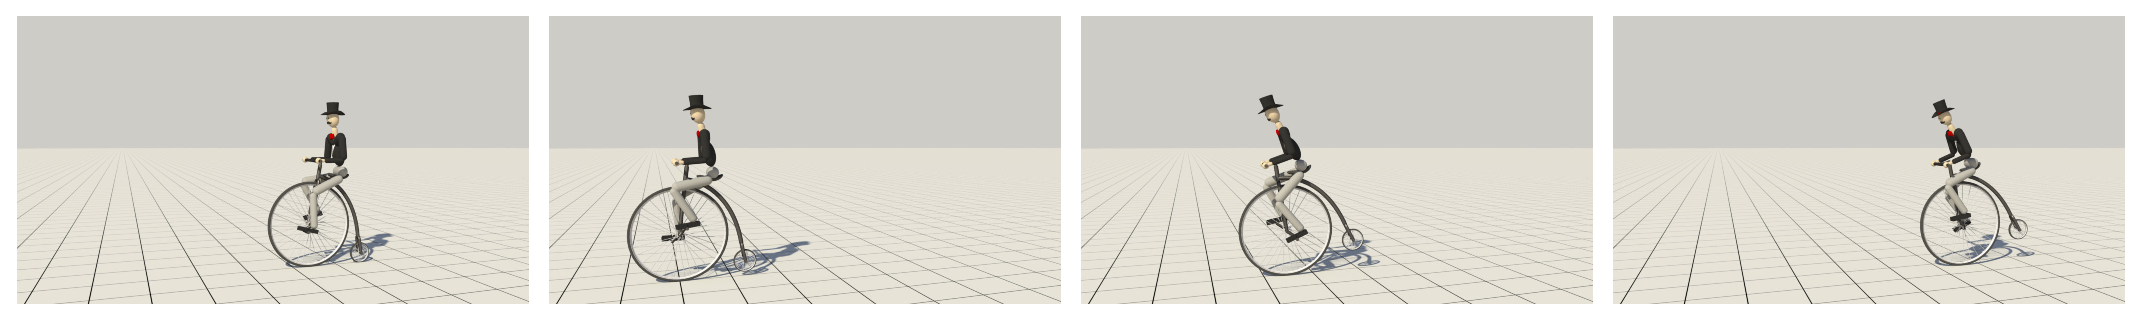
\includegraphics[width=\textwidth]{figures/velocipede}
\caption{A character rides a high wheeler and performs a stunt in which he rides backward on a single wheel.}
\label{fig:highwheeler}
\end{figure*}

\begin{figure*}[ht]
\centering
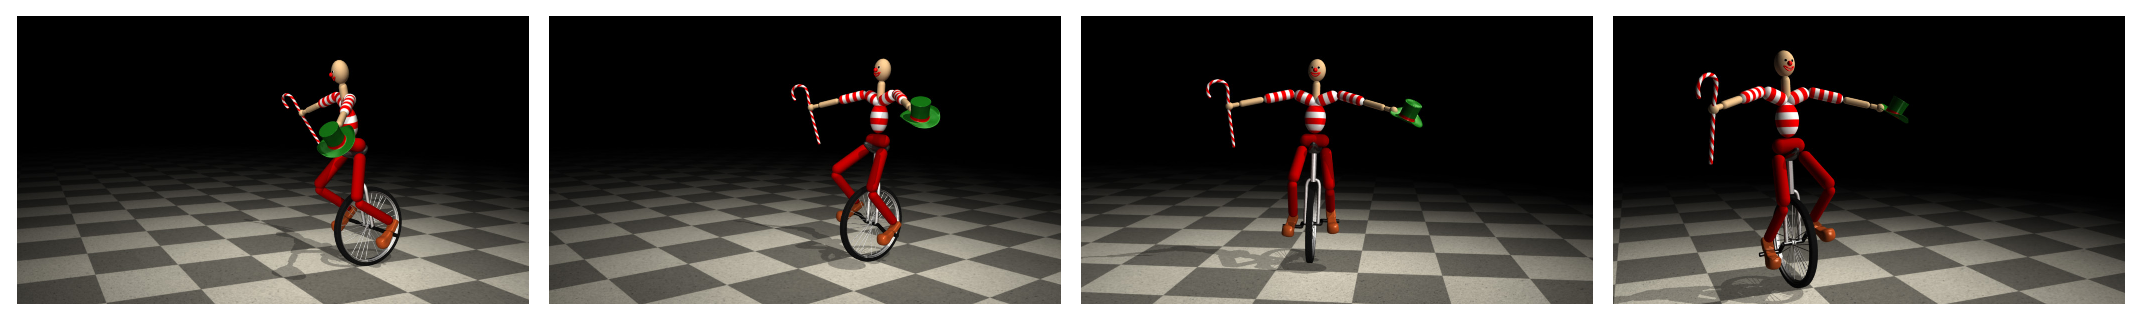
\includegraphics[width=\textwidth]{figures/unicycle}
\caption{A clown rides a unicycle.}
\vspace{-0.1in}
\label{fig:unicycle}
\end{figure*}

In this section we describe the results of our system. Please watch the accompanying video for the bicycle riding and stunt
animations. Our system was implemented in C++, and we used ODE with additional chain constraints to simulate both the bicycle and the human rider. The simulator runs in real time on a desktop workstation with a 2.26GHz CPU and 4GB of memory. We generated 90 samples per iteration and 50 iterations for offline policy search. The computations were distributed across 16 CPU cores on a cluster. The learning time ranges from a few minutes to half an hour depending on the number of simulations used to estimate the expected return (eq.~\ref{eq:policyValue}). Table~\ref{table:stateActions} summarizes the choices of states and actions for each bicycle task.

We designed three different bicycles and a unicycle to test our controllers on a variety of tasks. \emph{Road bikes} (Figure~\ref{fig:balance}) are designed to travel at speed on paved roads. They have very narrow tires to reduce the rolling resistance. The seats are mounted high so that the riders can bend their upper bodies down for less air resistance. We use a \emph{BMX bike} (Figure~\ref{fig:endo}) for stunts. BMX bikes are usually considerably smaller for nimble and agile handling. They have fat tires to facilitate balance and to increase traction. BMX bicycle parts can often be customized to meet the needs of different stunts. \emph{High wheelers} (Figure~\ref{fig:highwheeler}) are an old style of bicycle appearing in the late 19th century. They have a large front wheel and a much smaller rear wheel. This peculiar design makes high wheelers difficult to ride due to the center of mass being high and not far behind the front wheel. Any sudden stop could send the rider over the handlebars. A \emph{unicycle} (Figure~\ref{fig:unicycle}) has only one wheel and no handlebar. The rider needs to be concerned about the balance in both the longitudinal and the lateral directions. Different cycle designs greatly affect the handling characteristics and change the behavior of the riders. This variety puts the generality of our algorithm to the test. We modeled all the cycles and calculated their mass properties in SolidWorks.

\begin{table}[!b]
\vspace{-0.1in}
\centering
\begin{tabular}{|l|c|c|}
\hline
task & states & actions \\
\hline
momentum-driven & & \\
\hline
going over curbs      & $t, \beta$   & $\dot{v}_r, \tilde{\phi}$\\
endo (lifting)        & $t, \beta$  & $\tau_f, \tilde{y}, \tilde{z}$ \\
front wheel pivot     & $t, \dot{\gamma}$ & $\dot{\theta}, \tau_f, \tilde{y}, \tilde{z}$\\
bunny hop             & $t, h_f, h_r$ & $\tilde{y}, \tilde{z}$\\
\hline
balance-driven & & \\
\hline
balance and steering  & $\theta, \Delta \theta, \alpha, \dot{\alpha}$ & $\dot{\theta}$ \\
wheelie               & $\alpha, \dot{\alpha}, \beta, \dot{\beta}, \Delta \beta, v_r, \psi, \dot{\psi}$  & $\dot{v}_r, \dot{\psi}$ \\
endo (balance)        & $\theta, \alpha, \dot{\alpha}, \beta, \dot{\beta}, \Delta \beta$ & $\dot{\theta}, \tau_f$ \\
back hop              & $\alpha, \dot{\alpha}, \beta, \dot{\beta}, \Delta \beta, x, y, z$ & $\dot{x}, \dot{y}, \dot{z}$\\
high wheeler (stunt)  & $\beta, \dot{\beta}, \Delta \beta, \Delta v_f$ & $\dot{v}_f$\\
unicycle              & $\alpha, \dot{\alpha}, \beta, \dot{\beta}, v_r, \Delta v_r, \chi$ & $\dot{v}_r, \dot{\chi}$\\
\hline
 \end{tabular}
 \caption{Choices of states and actions for each bicycle task. Note that in the momentum-driven tasks, the actions only depend on time $t$ while the remaining states are used to compute the reward. }
 \label{table:stateActions}
 \end{table}

\paragraph{Balance and steering.} Riding a bicycle requires balance and steering. Balance can be maintained by steering toward the falling direction, which generates centrifugal force to push the bike upright. Figure~\ref{fig:balance} shows that our learned controller enables the rider to balance and steer the bike towards a user-specified direction. The bike follows the green arrow closely even when the user changes the desired direction abruptly. This agile steering behavior is achieved through ``counter-steering'': a momentarily steering in the opposition direction to initiate a sharp turn~\cite{Rankine1870}, which emerged automatically from the policy search. We also tested the robustness of our balance and steering controller on a bumpy terrain, which is represented as a noisy height field sampled from a uniform distribution $h\sim U(0, 0.05)$ (unit: meter). Even though the bicycle jumps and the handlebar is perturbed constantly, the rider still manages to balance and closely follows the desired direction. In addition, the accompanying video shows an initial starting motion, in which the rider's left foot is scripted to push the ground and move towards the pedal. Based on this single trajectory of foot and the learned balance policy, we used IK to generate the full-body motion of the starting phase.

\paragraph{Going down stairs.} Figure~\ref{fig:stair} shows the character riding down a series of stairs. Each step is 0.15m high and 0.8m wide. We used the same balance controller as in the previous example. This balance task is more challenging because the frequent loss of contact and the sudden collisions between the front tire and the ground narrow the window of effective control and introduce large perturbations. Initially, the rider needs to make large corrections with the handlebar to keep balance when the forward speed is low. As the bicycle travels faster, the corrections become smaller and steadier.
\vspace{-0.05in}

\paragraph{Going over curbs.} Riding over curbs (Figure~\ref{fig:curb}) can be performed by lifting the front wheel using feed-forward control only. We therefore parameterized the actions with two splines (Table~\ref{table:stateActions}) and trained the controller using CMA. We used a task-specific reward function to maximize the pitch of the bicycle $R_t = \beta$ during lifting. In the animation, as the bicycle approaches a curb (0.12m high), the rider first leans forward and then pushes her upper body backwards. When the arms are stretched out to the maximum length, the sudden deceleration of the upper body pitches the whole bike upwards. The pitch angle is further increased by pedaling faster. This sequence of highly coordinated movements is discovered automatically by the policy search algorithm. Once the front wheel goes over the curb, the balance controller takes over and keeps the bike upright when the rear wheel hits the curb.
\vspace{-0.05in}

\paragraph{Real time user interaction.} A user can interact with our bike simulation in real time. We video captured a sequence that shows a person using a joystick that is equipped with motion sensors to control the rider and the bicycle. The rider goes over a curb, survives a crosswind, goes down a set of stairs, and follows a curvy path to the goal. Note that the user only gives high level commands such as the desired steering angle and the timing of lifting the front wheel. The balance, the actual steering and the rider's motions are all controlled by the policy learned from the offline training process.
\vspace{-0.05in}

\paragraph{Wheelie.} A wheelie is a stunt maneuver in which the rider first lifts the front wheel and maintains balance on only the rear wheel. Lifting the front wheel on a BMX bike is considerably easier than on a road bike due to the shorter distance between the wheels. It can be achieved by increasing the speed of pedaling without any noticeable upper body movements. For this reason, we used only a feedback controller (Table~\ref{table:stateActions}) to perform a wheelie, including both the initial lift and the later balance. Once the front wheel leaves the ground, the rider adjusts the forward speed to keep the desired pitch angle. He leans his upper body to the left or to the right to correct any lateral instability.
\vspace{-0.05in}

\paragraph{Endo.} Figure~\ref{fig:endo} shows an endo. In contrast to a wheelie, an endo lifts the rear wheel and balances on the front wheel. In spite of its symmetry to a wheelie, an endo requires an entirely different set of skills and environments. Endos are usually performed on a gentle downward slope, which provides the needed forward momentum when the driving wheel is off the ground. We used a slope of 2.5 degrees in our example. We first search for a feed-forward controller that maximizes the negative pitch angle $R_t = -\beta$ to initiate the stunt. The resulting controller slowly moves the rider's pelvis to the back, and then quickly throws it to the front to lift the rear wheel.

The feed-forward controller is succeeded by a feedback balance controller. To maintain an endo, the rider continuously applies or releases the front brake for longitudinal balance and steers the handlebar towards the direction of leaning for lateral balance. This stunt is especially challenging. If the pitch angle is too large, when the COM is above or in front of the front tire contact, such a gentle slope cannot provide enough acceleration to prevent overturning. If the pitch angle is too shallow, to prevent the rear wheel from dropping to the ground, braking hard will quickly halt the bicycle and make the balance strategy of ``steering toward falling'' ineffective. This complicated coupling between the pitch angle, the speed and the lateral balance makes heavy demands on the policy search algorithm. NEAT successfully finds a policy that can maintain balance for an extensively long period of time. Figure~\ref{fig:simpleNetwork} Right illustrates the complex neural network required for this task.

In the accompanying video, we also demonstrate the learning process of an endo. The animation shows the resulting balance controller after one, five and ten iterations. As more iterations are finished, the rider gradually masters an endo and maintains balance for a longer period of time.

\paragraph{Front wheel pivot.} A front wheel pivot (Figure~\ref{fig:pivot}) is a fast way to turn the bicycle 180 degrees by pivoting on the front wheel. We used a feed-forward controller and applied two separate task-specific rewards during two phases of this motion. The first reward function maximizes the angle of turning during the pivoting phase.
\begin {displaymath}
\begin{array}{ll}
R_{t_1} = & \left\{ \begin{array}{ll}
\dot{\gamma} \Delta t & \textrm{if }h_r > 0.01,\\
0 & \textrm{otherwise.}
\end{array} \right. \\
\end{array}
\end {displaymath}
After the rear wheel touches the ground, we switch to a learned balance controller and measure how long the bicycle can stay balanced: $R_{t_2}=1$ if the bicycle remains upright. Without the second reward function, the ``optimal'' policy can produce a large roll during the pivoting phase, after which the rider cannot recover balance. In the animation, the rider performs an endo after turning the handlebar sharply to the left. As a result, the rider and the bike pivot around the front wheel and the 180-degree turn finishes within three seconds.
\vspace{-0.05in}

\paragraph {Back hop.} The back hop is another way to balance on the rear wheel. This feedback balance strategy uses small hops to change the relative position between the contact and the COM. In the animation, the rider and the bike start at an initial pose in which the COM is behind the contact point between the rear wheel and the ground. The bike will fall backwards if the rider does not correct for this. He bends his knees and then extends them to bring the rear wheel off the ground. He quickly pulls the handlebar towards himself in mid-air to adjust the pitch of the bicycle. When the rear wheel lands, the COM comes closer to the ground contact position. As a result, the rider can continue to hop and balance for a long time.
\vspace{-0.05in}

\paragraph{Bunny hop.} Figure~\ref{fig:bunnyhop} shows the rider performing a bunny hop on a BMX bike. A bunny hop is a stunt where the rider jumps with the bike over an obstacle or a trench. The task-specific reward function for the feed-forward controller is evaluated based on the height of both tires above the ground $R_t=h_fh_r$. Right before the hop, the rider first leans forward and then moves his pelvis rapidly towards the back of the bicycle. This vigorous motion tilts the bicycle upward. The rider then jumps with the bicycle over a clown lying on the ground. We were pleased to see that the optimal policy for the bunny hop motion includes a phase that tilts the bicycle up, which is essential to jumping for a greater height and distance. This style is known as the ``American bunny hop''.
\vspace{-0.05in}

\paragraph{Riding a high wheeler.} The peculiar design of a high wheeler makes ``headers'' a significant hazard, in which the rider gets pitch forward off the bicycle. We took on the challenge and designed a stunt that we had never seen performed on a high wheeler (Figure~\ref{fig:highwheeler}). During the stunt, the rider intentionally stops the bike to initiate a forward rotation. He then carefully changes pedaling speed to avoid taking a header and successfully rides backward on a single wheel. The rider can balance for a few seconds even without a lateral balance controller, probably due to the prominent gyroscopic effect from the large rotating front wheel. When the rider starts to lose balance, he accelerates to return to the normal riding mode, in which we used the same balance and steering controller as in the road bike examples.
\vspace{-0.05in}

\paragraph{Riding a unicycle.} The unicycle and the bicycle have many similarities. We have found that our algorithm is general enough to handle balance on a unicycle. Similar to some bicycle stunts, the longitudinal balance on a unicycle can be maintained via speeding-up or slowing-down, while the lateral balance can be maintained through steering toward falling. Unfortunately, unicycles do not have handlebars to steer. To steer the unicycle to the left, the rider needs to twist his upper body to the right. The unicycle will counter-rotate to the left due to the conservation of angular momentum. Figure~\ref{fig:unicycle} shows a clown riding a unicycle. To start riding, the clown first pedals backward, which leans the unicycle to the front. He then accelerates until the actual speed matches the user-specified desired speed. During riding, the clown repeatedly twists his waist to keep the lateral balance, which causes the unicycle to travel in a slightly sinusoidal path.



\section{Discussion and Limitations}
\label{sec:Evaluation}

\begin{table*}[ht]
\vspace{-0.1in}
\centering
\begin{tabular}{|l|c|c|c|c|c|c|c|c|c|}
\hline
task & wrist & elbow & scapula & shoulder & pelvis & hip & knee & ankle & ratio \\
\hline
\begin{tabular}{@{}l@{}}balance and \\steering (flat)\end{tabular} & 50 (5) & 150 (20) & 200 (30) & 550 (40) & 2000 (100) & 500 (150) & 500 (50) & 500 (50) & 0.9\\
\hline
unicycle & 10 (1) & 100 (5) & 100 (20) & 150 (10) & 2000 (30) & 100 (95) & 100 (90) & 60 (20) & 0.89\\
\hline
wheelie  & 10 (10) & 100 (30) & 100 (50) & 150 (80) & 2000 (100) & 500 (150) & 100 (100) & 60 (60) & 0.81\\
\hline
\begin{tabular}{@{}l@{}}going over \\curbs\end{tabular}& 50 (30) & 150 (50) & 200 (50) & 550 (80) & 2000 (100) & 500 (150) & 500 (100) & 500 (60) & 0.76\\
\hline
high wheeler & 50 (10) & 150 (50) & 200 (20) & 550 (200) & 2000 (300) & 500 (440) & 500 (360) & 500 (230) & 0.64\\
\hline
\begin{tabular}{@{}l@{}}balance and \\steering (bumpy)\end{tabular} & 50 (50) & 150 (100) & 200 (100) & 550 (350) & 2000 (400) & 500 (300) & 500 (350) & 500 (200) & 0.58\\
\hline
\begin{tabular}{@{}l@{}}front wheel \\pivot\end{tabular} & 250 (50) & 500 (150) & 500 (150) & 550 (400) & 2000 (600) & 500 (500) & 500 (280) & 500 (80) & 0.58\\
\hline
staircase & 50 (40) & 150 (100) & 200 (90) & 550 (350) & 2000 (400) & 500 (450) & 500 (450) & 500 (80) & 0.56 \\
\hline
bunny hop & 20 (15) & 50 (50) & 500 (150) & 550 (150) & 2000 (750) & 500 (400) & 500 (380) & 500 (220) & 0.44\\
\hline
endo & 50 (50) & 100 (100) & 100 (100) & 550 (400) & 2000 (600) & 500 (470) & 500 (485) & 500 (150) & 0.45\\
\hline
back hop & 250 (90) & 500 (400) & 500 (500) & 550 (545) & 2000 (900) & 500 (500) & 500 (450) & 500 (140) & 0.33\\
\hline
 \end{tabular}
 \caption{Torque limits (Unit: Nm) for different tasks. The values without the parenthesis are used for learning. The values within the parenthesis are the lowest torque limits that can be used in the simulation before the motion starts to fail. The amount of reduction is a measure of the robustness of the learned controllers. More reduction means a more robust controller. The last column reports the reduction ratios of average torque limits, which are sorted from high to low. This ranking is a possible indication of the difficulties (from low to high) that the learning algorithm think for each task. }
 \vspace{-0.1in}
 \label{table:torqueLimit}
 \end{table*}


Although the learning algorithms presented in this paper are general, the qualities of simulated motions vary with different tasks. We notice that some of the stunt motions do not look as compliant as those performed by real human riders due to three possible reasons. First, we chose large torque limits to allow robust control for various challenging maneuvers (Table~\ref{table:torqueLimit}). We used the same torque limits both in offline learning and online simulation to generate the results shown in the accompanying videos. To investigate whether we can achieve more compliant motions, we reduce the joint torque limits for simulation until the rider can no longer maintain balance (shown as the values in the parenthesis in Table~\ref{table:torqueLimit}). Although our controllers are robust when executed with smaller amount of torques, the resulting human motion appear very similar. The second possible reason is that we did not minimize rider's effort during offline learning. We found that it is difficult to weigh the effort minimization term because it competes with the task-specific objective. One possible solution is to implement prioritized optimization \cite{delasa:2009} to incorporate the effort minimization objectives. The last reason is probably due to the use of actuator constraints in ODE. The actuator constraints usually result in more stable simulation. However, since the joint torques are solved together with all other constraint forces, this allows the character to react instantaneously. We believe that the lack of reaction latency contributes to the stiffness of the motion. Using traditional PD servos could mitigate this problem but could also significantly increase the time of learning and simulation.


\begin{figure}[ht]
  \centering
  \includegraphics[width=3.4in]{figures/TorquePlot}
  \caption{Torque trajectories over time of performing an endo and riding a bicycle on a flat ground. }
  \label{fig:torquePlot}
\end{figure}

We further examine the torque trajectories (Figure~\ref{fig:torquePlot}), and observe that the controllers learned different strategies to achieve different tasks. In the endo example, the torques switch abruptly between the two extreme values. It is similar to the ``bang-bang control'' that frequently arises in time-critical tasks, indicating that the task of endo might also be time-critical. In contrast, the torque trajectory of riding a bicycle on a flat terrain shows more smooth transitions, which implies that normal biking does not require instant reactions and is thus an easier task.

\begin{figure*}[ht]
  \centering
  \includegraphics[width=\textwidth]{figures/NeatCMAComp}
  \caption{A comparison between policy searches with a fixed and an evolving parametrization. Left: The policy value vs. the number of iterations for ten policy searches on a fixed parametrization using CMA. Middle: Results of ten policy searches on a fixed parametrization using neuroevolution without augmenting topology. Right: Results of ten policy searches on an evolving parametrization using NEAT. }
  \label{fig:compare}
\end{figure*}

We have demonstrated that searching for both the parametrization and the parameters of a policy creates robust controllers for a wide variety of bicycle balance tasks. Since many previous studies focused on optimizing the parameters alone, we evaluated the necessity of optimizing the parametrization.
Figure~\ref{fig:compare} Left and Right compares two policy search results with a fixed and with an evolving parametrization for the balance task of an endo. Both searches started with the same parametrization: a neural network with direct connections between the input and the output layers. We used CMA to search for only the weights while we used NEAT to evolve both the weights and the network structure. Both algorithms were run for 50 iterations with 90 samples per iteration. We ran each search ten times with different random seeds to reduce the stochastic bias. Figure~\ref{fig:compare} Left plots the curves of the policy value versus the number of iterations in the CMA search. Note that none of the searches reached a value of 3000. In comparison, eight out of ten NEAT searches found policies scored higher than 3000 (Figure ~\ref{fig:compare} Right). Three of them reached almost 7000. The average final policy value of NEAT was almost twice its CMA counterpart. A similar comparison was conducted between neuroevolution with and without augmenting topology, and this told the same story (Figure~\ref{fig:compare} Middle vs. Right). Even though we only reported the detailed comparison for this particular example, we observed the same trend for other bicycle stunts: policy search with an evolving parametrization significantly outperforms search with a fixed parametrization. The neural network structure for all the balance-driven tasks are shown in the supplementary material.

As illustrated in Section \ref{sec:results}, many bicycle stunts need balance in both the longitudinal and lateral directions. In our implementation, we decoupled the balance task in these two directions and learned the task in two steps. In the first step, we focused on longitudinal balance and chose only the relevant states and actions. We artificially increased the width of the tire to 20cm so that the controller did not need to be concerned about the loss of balance in the lateral direction. This is analogous to using training wheels in real life. Once the longitudinal controller had been learned, we fixed that part of the neural network, reduced the width of the tire back to normal\footnote{The tire width of the road bike and the high wheeler is 1.5cm while the tire width of the BMX bike and the unicycle is 3cm.} and then performed the second step of training for lateral balance. Although in theory, optimizing a controller for the longitudinal and the lateral balance simultaneously would have a better global optimum, in practice, searching for a policy in a higher dimensional space is subject to local minima and thus could produce inferior results. In all our examples, this two-step training found better policies than training both longitudinal and lateral balance simultaneously.

Our attempts at learning bicycle stunts using other reinforcement learning algorithms ended up unsuccessful, but these valuable experiences led us to our current solution. Our first attempt was to use standard value iteration method with a discretized state space. The high dimensional state space made the tabular representation infeasible. We encountered the convergence issue when the state space was parameterized by polynomial and Gaussian kernel bases. We also experimented with a few model-free learning algorithms. For example, SARSA($\lambda$) demonstrated some potential (\ie the normal cycling was successful), but the computation time was too long even for the simplest task. Although our final decision was to use policy search, the initial experiments were unsuccessful due to an overly simplified policy parametrization: a neural network without hidden layers. Using quadratic features to enrich the inputs of the network, we had some limited success with the optimal solutions solved by CMA. However, without a systematic way to perform feature selection, the likelihood of finding a successful local minimum is low due to the large number of quadratic features. Finally, we chose NEAT, a bottom-up approach that complexifies the parametrization from the simple network. This method consistently found policies that worked for all our examples.

NEAT provides an effective way to search for both the parametrization and the parameters, which frees us from laborious and unintuitive manual tuning of the network structure. However, to formulate an MDP, we still need to design the state space, the action space and the reward function. While designing the state space is often straightforward, choosing appropriate actions for a specific task requires domain knowledge. For example, knowing how to steer a unicycle is essential for the unicycle balance task. Likewise, designing a good reward function requires some trial-and-error experiments. Our reward functions initially contained only the task-specific terms. We found that the algorithm often discovered a policy that had a high value but resulted in undesired motions: The rider performed redundant movements as long as this did not affect the balance. We eliminated these undesired motions by adding regularization terms to the reward function. However, selecting states, actions and reward functions is unavoidable when formulating and solving MDPs. Inverse reinforcement learning \cite{Ng:2000} might be a promising approach, but this requires data generated from the optimal policy, such as motion capture data from real stunt bikers. Compared to manually designing a policy parametrization, learning the domain knowledge and tuning the reward function is more intuitive and fun.

Our system has a few limitations. We used ball joints to attach the feet to the pedals. These bilateral joint constraints simplify the simulation but render some motions less realistic: The brief moment in our bunny hop animation when the rear wheel pops off the ground just before the hop typically is not seen in the real stunt. Faithfully modeling the contact between the feet and the pedals could solve this problem. However, this will make the simulation more expensive and the learning more difficult. In the learning, we separated the feed-forward and feedback controllers. This treatment works well if the feed-forward controller is applied for a short period and then we switch to the feedback controller. However, in a real-life performance, stunt bikers exhibit both feed-forward and feedback controls at the same time, which allows them to perform longer and more difficult stunts. This might be one of the reasons that our algorithm cannot generate a 360-degree front wheel pivot. Our interactive simulation does not allow the user to arbitrarily concatenate the stunts. Successful stunts demand a stable initial pose, appropriate speed and sometimes a favorable terrain. All these requirements together prevents us from concatenating stunt controllers arbitrarily. Learning additional intermediate controllers between stunts might be a possible solution.

\section{Conclusion}

We have presented an algorithm for animating bicycle stunts.  Key aspects of our approach include a fast and stable physical simulation,
policy search for POMDP, and
the use of a sample-based optimization solver that searches for both the structure and the weights of a neural network.
Our system allows us to control a human character that
performs a variety of bicycle stunts, including wheelie, endo, bunny hop, front wheel pivot and back hop.
Our characters can learn to master the most demanding balance tasks in minutes, which challenges most people and takes months of practice to learn.

Policy search is a powerful method for learning optimal controllers. However, manually designing parametrization of the policies could be challenging for difficult tasks. Combining policy search with NEAT makes it easy to use and unleashes its full power. We believe that its success will not be limited to the bicycle control tasks. It has the potential to solve other challenging control problems, such as gymnastics, skateboarding, surfing and dancing.

There are a number of interesting avenues for future work. Deep learning \cite{Hinton:2007} and deeper neural networks could be explored for even more difficult stunts. Our work has concentrated on controllers for individual stunts. It would be interesting to investigate a sequence of stunts that traverse a bicycle course with obstacles. Finally, it would be fascinating to manufacture a mini bicycle and a robotic rider and apply our controllers to make them perform stunts in the real world.
